\noindent
{\bf Collaborative Research: Mathematical modeling and simulation of
self-assembling amphiphilic particles in solvent {\bf MAKE MORE MATHEMATICAL}} \\
{\em Rolf Ryham (lead PI, Fordham University),
Bryan Quaife (PI, Florida State University), and
Yuan-Nan Young (PI, New Jersey Institute of Technology)}

\section{Background}
\label{sec:background}

Mathematical models of self-organization encompasses a
broad range of interesting and challenging phenomena.
For example, understanding the organization of lipids and proteins in vesicles
is crucial to design effective drug and vaccine carriers.
The COVID-19 pandemic has lead to an unprecedented and concerted worldwide
effort in biophysical modeling of the mechanisms of RNA condensation
by structural proteins, protein oligomerization, and cellular
membrane–protein interactions that control ultimate virus structure,
in an effort to curtail pathogens like the Severe Acute Respiratory Syndrome Coronavirus 2.
Using powerful capillary and van der Waals forces that exist at the nanoscale, engineers
have developed superior techniques to print 
high-resolution, nanoscale features on devices like sensors, lasers, and LEDs.
Finally, researchers have introduced data-driven methods 
to study complex patterns that emerge in particle and agent-based systems like swarms
and flocking.

A number of mathematical techniques have beed developed to handle
self-organizing systems.  Each technique has its advantages and disadvantages.
Prominent in chemistry and biology, molecular
dynamics (MD) simulations offers unparalleled resolution of protein-lipid interactions,
say, but because of the large number of non-linear interactions involved,
is limited to short time and small spatial scales.
In terms of inverse problems,
agent based systems also involve relatively large numbers of particles
and here researchers extensively consider the problem  
of learning interaction kernels in these dynamical systems
constrained to evolve on Riemannian manifolds from given trajectory data.
Once the interaction kernels are known, one can in principle derive
partial differential equations (PDE) for the macroscopic behavior. 

The phase field method and self-consistent field theory are popular  
approaches to self-organization in applied mathematics.
Motivated by Ginzburg-Landau theory, these methods introduce a scalar-valued
phase field function for the volume fraction of
lipids and water in modeling vesicles membranes, for example. 
Sometimes called diffuse interface methods, here one devises energy functionals
involving the gradient and well-potentials of the phase field, and possibly
long range interaction kernels, that yield approximate mathematical surfaces
of almost arbitrary topology.
Because the fluid interfaces are given by the level-set
of a smooth function, the evolution equations
can be studied by well-established tools like variational methods
and regularity theory, and are amenable to numerical approximation.
On the downside, granular details like the shape changes of a protein, for
example, are clumsy to incorporate in the model.  Moreover, numerical
simulations of phase field models typically discretize the entire fluid
domain under consideration, and apply cutoff boundary conditions
when periodic domains are not under consideration. 

(Surface-director models.)

\begin{figure}
  \begin{center}
    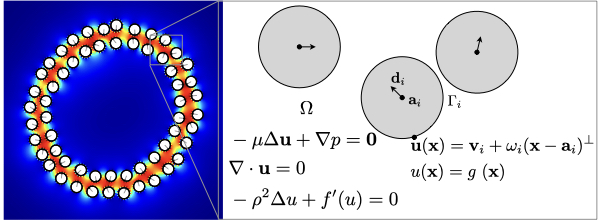
\includegraphics[width=0.45\textwidth]{figures/SpecificAim1/Domain.jpg}
% 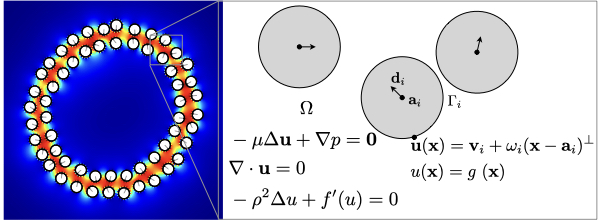
\includegraphics[width=0.55\textwidth]{figures/SpecificAim1/Domain.jpg}    
 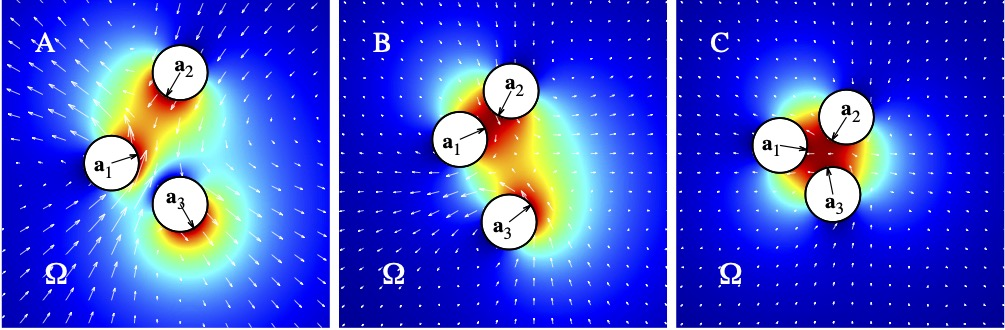
\includegraphics[width=0.45\textwidth]{figures/SpecificAim1/3Particles.jpg}
  \end{center}
  \caption{\label{fig:flow_map}
   Left: In the HAP formulation,
   a system of exterior problems 
   defines the hydronamic and hydrophobic interactions.
  Right:
     Particles translate and rotate to lower the free energy $F[u]$
   subject to \eqref{eq:SL}, $f(u) = u^2$, and reach a minimal configuration in
   panel C. The colormap is blue for $u = 0$ and red for $u = 1$.
   The arrows are the velocity field $\mathbf{u}$.}
\end{figure}



Recently, we have developed a new mathematical model of self-organization.
The model takes ideas from the phase field method 
and leverages boundary integral equations to speed up computations.
To formulate the problem, consider a collection of $N_b$-many rigid bodies
$U_i$ immersed in an incompressible, zero-Reynolds number fluid
$\Omega_t \mathbb{R}^n \setminus \cup_{i=1}^{N_b} U_i$.
The subscript $t$ reinforces that $\Omega_t$ is time-varying. 
We use the grain shape and boundary conditions to capture the local 
properties of the suspended media.
Unlike particles, the bodies, which we will call grains (``using `grains' as an easy find-replace for
when we settle on vocabulary), have finite size.

The first key idea is
to define the grain interactions using a boundary value problem
\begin{align}
  -\mu\Delta \uu + \nabla p &= \mathbf{0},\\
  \nabla \cdot \uu &= 0,\\
-\rho^2 \Delta \eta + f'(\eta) &= 0, \quad \text{ in } \Omega_t,
\end{align}
with boundary conditions
\begin{align}
  \frac{d\xx}{dt} &= \uu,\\
  \uu &= \vv_i + \omega_i \times (\xx - \aa_i)\\
  \eta &= h_i(\xx,t),\quad \text{ for } \xx \in \Gamma_i
\end{align}
and
\begin{equation}
\int_{\Gamma_i} \mu(\nabla \uu + \nabla \uu^T + pI)\nu \,\dif s = 
\int_{\Gamma_i}
\underbrace{(-\rho^{-1} f'(\eta)
  + \rho(\tfrac{1}{2}|\nabla \eta|^2 - \nabla \eta \nabla \eta^T)}_{T_i} \nu \, \dif s
\end{equation}
This is a semi-linear system for evolution of the grains.  At the top,
the Stokes equations describe the velocity $\uu$ and pressure $p$ of the
aqueous phase. In third equation describes the phase transitions of the
scalar order parameter $\eta$ with a decay length $\rho.$
Mathematically, this order parameter is responsible for the attraction
and adhesion between grains that want to align boundaries of like phase.  
Physically, water molecules are polar and $\eta$ describes the orientational
order of water e.g. $\eta = 1$ when water molecules share alignment
and $\eta = 0$ when the water orientations are disordered.
The well-potential $f$ accounts for possibly distinct equilibrium phases,
as occurs with 3-bond and 4-bond hydrogen bonding.

The next three equations are the moving domain boundary conditions.
The first two specify a non-slip boundary condition for a rigid body
with translation velocity $\vv_i$ and angular velocity $\omega_i$.
In the third boundary condition, the function $h_i$ is a material label
speficying the water phase at the water-grain interface.  This material
label is transported by the fluid and therefore satisfies $h_i(\xx,t)
= h^0_i(\xx(\XX,t),t)$ where $h_i^0$ and $\XX$ are reference labels, coordinates
given by the initial conditions, and $\xx(\XX,t)$ is the flow map for the
rigid bodies.  Finally, the last boundary condition closes the system
and says that the hydrodynamic stress is balanced by the water-order stress.

Intriguingly, the formulation ()-() captures exactly the right behavior
expected from amphiphilic self-assembly.  Three bodies with amphiphilic
label spontaneously translate and change orientations to sequester the
disordered fluid phase.  In our simulations (see section ()), we include
a finite length repulsion to avoid particle collisions.
Moreover, a simple change of boundary conditions from amphiphilic,
to biased hydrophobic, to polar results in distinct equilibrium morphologies.

\begin{figure}[h]
  \begin{center}
    \begin{tabular}{m{0.1cm}m{1.8in}m{1.8in}m{1.8in}}            
      (a)
    &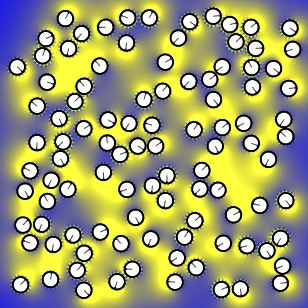
\includegraphics[width=1.8in]{figures/SpecificAim1/N100B1.jpg}
    &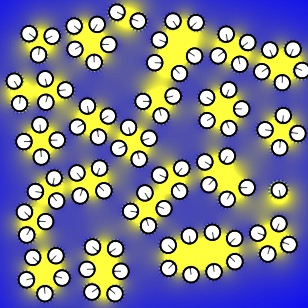
\includegraphics[width=1.8in]{figures/SpecificAim1/N100B2.jpg}
     &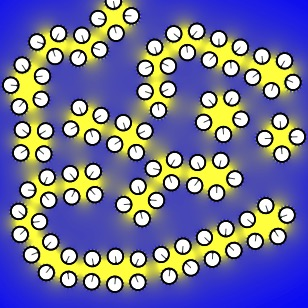
\includegraphics[width=1.8in]{figures/SpecificAim1/N100B3.jpg}    \\
     (b)
    &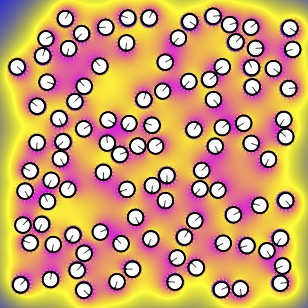
\includegraphics[width=1.8in]{figures/SpecificAim1/N100C1.jpg}
    &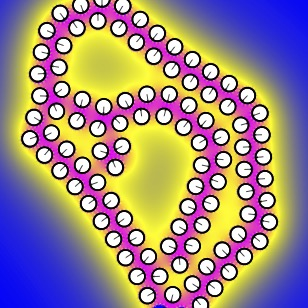
\includegraphics[width=1.8in]{figures/SpecificAim1/N100C2.jpg}
      &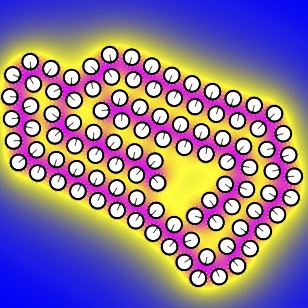
\includegraphics[width=1.8in]{figures/SpecificAim1/N100C3.jpg}    \\
    (c)
      &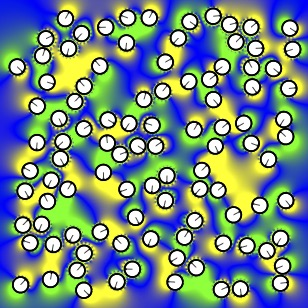
\includegraphics[width=1.8in]{figures/SpecificAim1/N100A1.jpg}
      &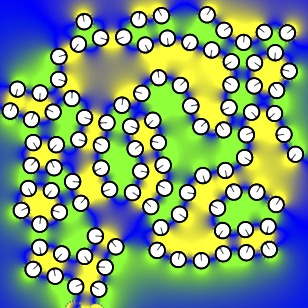
\includegraphics[width=1.8in]{figures/SpecificAim1/N100A2.jpg}
      &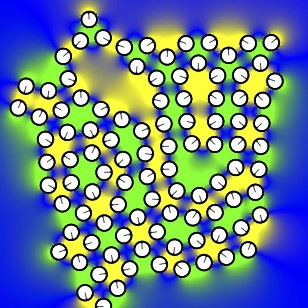
\includegraphics[width=1.8in]{figures/SpecificAim1/N100A3.jpg}    \\
      &\multicolumn{1}{c}{$t = 0$}
      &\multicolumn{1}{c}{intermediate time}
      &\multicolumn{1}{c}{long time}
  \end{tabular}
  \end{center}
  \vspace{-20pt}
  \caption{\footnotesize
    \label{fig:self-assembly}
    Rows (a)-(c) have the same initial configuration
    but have different boundary conditions $g.$ 
    In row (a), self-assembly with an amphiphilic boundary
    condition \eqref{eq:bcs}(a) results in a bilayer pattern shielding
    the hydrophobic core (yellow, $u > 0$) from the aqueous phase (blue, $u = 0$).
    Row (b) shows particles with a hydrophobic intensity that is
    greater on one side of the particle (magenta) than the other (yellow).
    In row (c), green is for $u < 0$, yellow is for $u > 0$, and blue is for $u = 0$.
    Particles orient like sides to form a checkerboard pattern.\\
  }
\end{figure}


The system ()-() has an elegant mathematical structure.
In terms of locally in time well-posedness, given disjoint grains with
sufficiently smooth boundaries
and data, the system ()-() always has a solution and that these solutions
have a locally Lipschitz dependence on the particle centers and orientations. 
Solutions of ()-() obey the energy law
\begin{equation}
  \frac{d}{dt}F
  = - \int_{\Omega_t} \tfrac{1}{2}\mu|\nabla \uu + \nabla \uu^T|^2 \,dx,
  \quad
  F = \int_{\Omega_t}
  \rho |\nabla \eta|^2 + \rho^{-1} f(\eta) \,dx.
\end{equation}
Mathematically, this energy law states that the free energy $F$ of the water order
phase transitions, which depends on the grain configurations, is lost due to
hydrodynamic dissipation.  It is evident that minimizers of the functional $F$
are unique and satisfy the Euler-Lagrange equation ().
There is a subtlety in the energy law, though.  Namely, the
time derivative of the free energy $F$ also involves the moving
boundary, accounted for by the Rayleigh Transport Theorem, and the
fact that the boundary data for $\eta$ are transported by the rigid body motion.
In fact, the water order surface stress $T_i$ is the variational derivative that
shows up in this calculation.

The model has a broad range of applicability to self-organization phenomena
in chemistry and biological physics. Since the formulation is
scale independent, it can represent a suspension of amphiphiles,
where the grains represent
the mean properties of a small collection of lipids, at the nanoscopic scale.
For larger scales, the representation is literal and the grains Janus spheres.  
The proposal deals with the physical origins in section (). 

To summarize, the formulation ()-() shares a lot of the features in phase field modeling,
with the big exception that the free energy depends on the grain configurations,
rather than phase field
function.
To make an explicit connection though, we can consider a phase field model 
where one ``fluid'' phase instantaneously reaches minimality while the other ``solid''
phase moves to further decrease free energy. 
The model is also closely related to
a recent and strongly developing direction studying 
colloids immersed in nematic liquid crystals.
As is the case for nematics, it is natural to understand what is the effect of the flow in
such a context, but a first step is to obtain some solid well-posedness results.
The proposal discusses some mathematical generalizations in section ().  

The boundary integral equation (BIE) method is
the idea numerical method for the present study
in terms of computational cost and accuracy.
Boundary integral equations
require linear PDE and so we take $f(\eta) = \tfrac{1}{2}\eta^2$,
yielding in () the so called screened Laplace equation
$-\rho^2 \Delta \eta + \eta$.  This is a Helmholtz equation with purely imaginary
wave number, enabling us to represent the solution
in terms of layer potentials:
\begin{equation}
  \eta(\xx) = \int_{\partial \Omega} \frac{\partial G}{\partial \nu}
  \left(\frac{\xx-\yy}{\rho}\right) \sigma(\yy) \,ds_{\yy}
\end{equation}
where $\frac{\partial G}{\partial \nu}$ is the normal derivative of the
fundamental solution of the screened Laplace equation
(a Bessel function in two space dimensions and
an exponential times the standard fundamental solution of the Laplace equation
in three space dimensions).
This representation allows us to transfer the boundary value problem ()-()
to an equation only involving in terms of domain boundary.  

The numerical advantages of doing so are as follows.  If $h = N^{-1}$
is the characeristic grid spacing of the grain boundaries, then a
finite element or finite difference discretization of ()-()
requires on the order of $N_b N^n$ grid points
for dense suspensions.  In contrast BIE require onely 
With finite elements, mesh regeneration
would be needed at each time step since the domain is moving.  
In the boundary integral approach, collocation points can be selected
for the initial grain configuration and then used throughout the
time-course.
As a downside, integral equations require specialized quadrature
routines to resolve self interactions and nearly touching
grain boundaries.  
Finally, the far field boundary conditions which are important for
imposed flow problems automatically hold, whereas with 
finite element and finite difference methods
artificial boundary conditions must be imposed.
\begin{figure}
A figure comparing FE versus BIE meshes
\end{figure}

\subsubsection{Problem formulation}
%\begin{wrapfigure}[h!]


The mathematical formulation is a nonlinear system for the dynamics of a
collection of particles. The interactions come from a system of 
partial differential equations (PDEs) that comprise hydrodynamic
interactions and hydrophobic interactions.
%The formulation prevents particle collisions through excluded volume
%potentials. 
The hydrodynamic interactions come from the mobility problem for rigid
particles immersed in a viscous solvent. We then use a
second-order Adams-Bashforth method to update the particle configuration.
Assuming inertial terms are
negligible, the particle motion is goverened by the Stokes equations
\begin{subequations}
  \label{eq:stokes}
  \begin{alignat}{3}
  \label{eq:stokes1}
  -\mu \Delta \uu + \nabla p &= \mathbf{0}, && \xx \in \Omega, \\
    \label{eq:stokes2}
  \nabla\cdot \uu &= 0, \qquad && \xx \in \Omega, \\
\label{eq:stokes3}
  \uu - \uu_\infty &\to \mathbf{0}, && |\xx| \to \infty,
  \end{alignat}
\end{subequations}
%\begin{alignat}{3}
%\label{eq:stokes1}
%  -\mu \Delta \uu + \nabla p &= \mathbf{0}, 
%    && \xx \in \Omega, \\
%\label{eq:stokes2}
%  \nabla\cdot \uu &= 0, \qquad && \xx \in \Omega, \\
%\label{eq:stokes3}
%  \uu - \uu_\infty &\to \mathbf{0}, && |\xx| \to \infty,
%\end{alignat}
%
where $\uu$ is the velocity and $p$ is the pressure of the solvent,
$\uu_\infty$ is the background flow, and $\mu$ is the constant solvent
viscosity. The domain $\Omega = \Omega(t)$ is the fluid region surrounding the
particles and changes shape as the particles move.
Since the particles are rigid, the solvent velocity satisfies
a no-slip boundary condition for a rigid body motion 
%\begin{align}
%\label{eq:rigid_bc}
%  \uu(\xx) = \vv_i + \omega_i  (\xx - \aa_i)^\perp, \quad
%    \xx \in \Gamma_i,\qquad  i=1,\ldots,N_p,
%\end{align}
on the particle boundary $\Gamma_i$ with translational velocity $\vv_i$
and angular velocity $\omega_i$ (Figure \ref{fig:flow_map}).
Given imposed forces acting on each
particle, the \emph{mobility problem} consists of finding
translational and angular velocities so that viscous fluid forces
balance the imposed forces.

The hydrophobic interactions come from the tendency of particles to
minimize the free energy of the structure of the surrounding water
molecules. The free energy functional takes the form 
\begin{equation}
\label{eq:free_energy}
  F[u] = C \int_{\Omega} \left(\rho |\nabla u|^2 + \rho^{-1} f(u)\right)
  \,d\xx,
\end{equation}
where $u$ is an order parameter for the structure of water, $\rho$ is a
decay length, $C$ is a constant, and $f(u)$ is a potential.
Hydrogen-bond persistence times are on the order of picoseconds
which is much smaller than characteristic time for 
particle motion \cite{MaGa13}.
Thus we assume $u$ minimizes $F[u]$ for all times.
Assuming appropriate conditions on $f(u)$ (\cite{evans10}, \S 8.2),
$u$ is bounded and satisfies the Euler-Lagrange equation
\begin{equation}
\label{eq:SL}
-\rho^2 \Delta u + \tfrac{1}{2}f'(u) = 0  \text{ in } \Omega,\quad u = g,
\text{ on } \bd\Omega.
\end{equation}
The boundary condition $g$ is a material label that is transported with
the particle (Figure~\ref{fig:bcs}).

The particles lower the free energy $F[u]$ of the surrounding water
by moving. We calculate the rate of change of $F[u]$ using
\emph{variation of the domain} ~\cite{Fu2018_SIAM,Bandle2015, Schiffer1954, Grinfeld2010}.
Carrying out
this variation yields a 
%The hydrophobic forces are torques are
%\begin{equation}
%  \label{eq:hydrophobicAttraction}
%  \FF_i^{\text{hydro}} = \int_{\Gamma_i} {\bf T}\cdot \nnu \, \dif s, 
%    \quad 
%    T_i^{\text{hydro}} = \int_{\Gamma_i} (\xx - \aa_i)^{\perp} \cdot
%    ({\bf T} \cdot \nnu) \dif s.
%\end{equation}
stress  
\begin{align}
  \label{eq:stress}
\mathbf{T}
= C \left[ \rho^{-1} f(u) \mathbf{I}
  + \rho \left(|\nabla u|^2 \mathbf{I} - 2\nabla u \nabla u^T\right)\right].
\end{align}
The imposed forces and torques come from the integration of $\mathbf{T}$
along the particle boundary.
These forces and torques couple the Stokes equations \eqref{eq:stokes},
to semilinear elliptic equation \eqref{eq:SL}.
Solving for the translational and rotational velocities gives the
particle evolution.



The stress~\eqref{eq:stress} was first
introduced by~\cite{Fu2018_SIAM} and is the higher-dimensional
generalization of disjoining pressure \cite{MaRa76, ErLjCl89, KoNa15,
Nagle17, KUZMIN2005}. It is the mathematical ingredient responsible for
forming particle aggregates that sequester their hydrophobic surface
regions (Figure \ref{fig:3particles}).

%By solving the above system, we obtain translational and angular
%velocities of the many-body system. A second-order Adams-Bashforth
%scheme updates the particle positions and orientations.

The formulation presents a number of mathematical and numerical
challenges. For one, the domain is constantly changing so that a new
boundary value problem must be solved at each time step. The particle
boundaries are nearly touching and high-order numerical
schemes and adaptively chosen time-step sizes
are required to calculate trajectories accurately.
Furthermore, the domain is unbounded and care must be taken 
in capturing the far-field boundary conditions correctly. 
Finally, the numerical routine must handle large system sizes
efficiently.

%and
%\begin{equation}
%  \label{eq:force}
%  \int_{\Gamma_i} \ssigma \cdot \nnu \, \dif s = \FF_i,\quad 
%  \int_{\Gamma_i} (\xx - \aa_i)^{\perp} \cdot (\ssigma \cdot \nnu) \,
%  \dif s = T_i, \qquad i=1,\ldots,N_b,
%\end{equation}
%where
%$\ssigma = -p \mathbf{I} + \mu \left(\nabla \uu + \nabla \uu^T \right)$
%is the hydrodynamic stress tensor (pressure tensor) and $\nnu$ is the
%particle outward normal.

\subsection{Boundary Integral formulation}
\textbf{Take from prior years proposal}


\subsection{Outline of the proposal}
